\documentclass[aps,prc,twocolumn,showpacs,floatfix,nofootinbib,preprintnumbers,superscriptaddress,amsmath,amssymb]{revtex4-1}

\usepackage{wrapfig}

\bibliographystyle{apsrev}

\ifx\pdfoutput\undefined
\usepackage[dvips]{graphicx}
\else
\usepackage[pdftex]{graphicx}
\pdfcompresslevel=9
\fi
\usepackage{epstopdf}


\def\psibar{\overline{\psi}}
\def\chibar{\overline{\chi}}
\def\mcC{\mathcal{C}}
\def\mcN{\mathcal{N}}
\def\mcO{\mathcal{O}}


\newcommand{\OP}[1]{{\bf\widehat{#1}}}

\newcommand{\be}{\begin{equation}}

\newcommand{\ee}{\end{equation}}

\begin{document}

\pagestyle{plain}

\section*{Aspects and applications of the gradient flow in lattice QCD: 
strong coupling, electric dipole moments and strange content of the nucleons}

The Standard Model of Particle Physics (SM) has been widely successful in describing 
the measured particle spectrum and composition of matter ranging from quarks and gluons 
to multi-hadron systems.  Such systems constitute approximately 5\% of the observable 
matter-energy within the Universe.  Yet the theory alone cannot explain the origins of 
the remaining 95\% of matter and energy, dubbed `Dark Matter' and `Dark Energy', respectively.  
Further, the SM does not provide the requisite amount of charge conjugation and parity (CP) 
symmetry violation to account for the observed matter/anti-matter asymmetry.  Therefore any physical description of such 
phenomena requires a theory that goes \emph{beyond} the Standard Model (BSM), while at the 
same time encompassing the Standard Model and its predictions related to ordinary matter.

There are numerous candidate BSM theories and a description of these theories is 
beyond the scope of this project.  However, these theories all share certain operator 
traits that can be utilized in a formal study involving numerical methods of 
quantum chromodynamics (QCD), the gauge theory describing the strong interactions.  
When viewed as a low-energy effective theory of some larger (still unknown) fundamental theory, 
the SM, consisting of renormalizable operators of dimension 4 or less, 
is augmented with BSM operators of dimension $>$ 4.  The structures of these higher 
dimensional operators can be determined generically assuming the larger fundamental theory 
respects certain symmetries (e.g. the combined charge conjugation, parity and time reversal (CPT) invariance). 
Different candidate BSM theories will give different couplings for these higher-dimension operators.  When BSM theories 
are expressed in this manner, all the benefits inherent to effective field theories (EFTs) follow through, 
such as a hierarchy in operator complexity and a systematic power counting of terms.

Because of the generality of these higher-dimension operators, 
calculations of these operators can be performed with their unknown coefficients as free parameters using lattice QCD (LQCD), 
to be later fixed by candidate BSM theories.  
Conversely, a phase-space investigation of these parameters can be studied to rule-out different BSM theories.  
The study of these higher-dimension operators with a lattice regulator is plagued by 
hard renormalization ambiguities. 
The lattice discretized version of these higher-dimension operators can cause mixing of their coefficients 
with lower-dimension operators, making the separation and extraction of BSM observables from standard QCD observables very difficult.  
To address this issue, we have proposed a new method~\cite{Shindler:2014oha,Shindler:2015aqa} 
based on the use of the gradient flow~\cite{Luscher:2010iy,Luscher:2013cpa} 
to circumvent such mixing, as well as to address other issues related to renormalization.

The overall goal of this research program is to calculate nuclear observables induced by these general BSM operators using lattice QCD.  
Such observables include the electric dipole moment of nucleon and few-body nuclear systems
and the strange content of nucleons. 
In this thesis project we focus on the pertubative calculations needed 
to match the results obtained and non-zero flow time with the physical results.

\section*{Strange content of a nucleon}

A very popular example of dark matter (DM) candidate is a  
weakly interacting massive particle (WIMP) like the ones that are predicted in 
a large class of models~\cite{Bertone:2004pz}.
Definite evidences for a direct detection of WIMPs have only been recently suggested, with various ongoing experiments providing rather severe constraints for the parameters of many DM models. 

A possible scenario for the detection of a WIMP type of DM particles relies on the idea  
that the WIMP, due to its assumed large mass, produces a Higgs boson 
that couples to the various quark flavor scalar density operators taken
between nucleon states (see fig.~\ref{fig:wimp_N_scatt}). 
At zero momentum transfer, the cross section for spin independent elastic WIMP--nucleon ($\chi N$) 
scattering reads \cite{Ellis:2008hf}

%
\begin{equation}
\sigma_{\chi N} \sim  
\Big\lvert\sum_{f} G_f(m_\chi^2 ) f_{T_f} \Big\rvert^2  \qquad \text{with} \qquad f_{T_f} 
= \frac{m_{f}}{m_N} \left\langle N | \bar{q}_f{q_f} |N \right\rangle \, .
\label{eq:crosssection} 
\end{equation}
%
The functions $G_{f}$ depend on several parameters of 
the particular BSM theory used for the calculation of
$\sigma_{\chi N}$, which include the WIMP mass, $m_\chi$. 
The dimensionless and renormalization group 
invariant (RGI) coupling $f_{T_f}$ depends on the mass $m_{f}$ of the quark 
of flavor $f$ and the nucleon mass, $m_N$.  As evident from Eq.~(\ref{eq:crosssection}), the cross section, $\sigma_{\chi N}$ 
depends quadratically on $f_{T_f}$, and is therefore very sensitive 
to the size of the scalar content contributions of different flavours. A O(10\%) variation
of $f_{T_f}$, for example, can lead to significant changes in $\sigma_{\chi N}$. 
It is therefore necessary to compute accurately and with controlled error 
the hadronic matrix elements $\left\langle N | \bar{q}_fq_f |N \right\rangle$.   

 %
\begin{figure}[tb]
\begin{center}
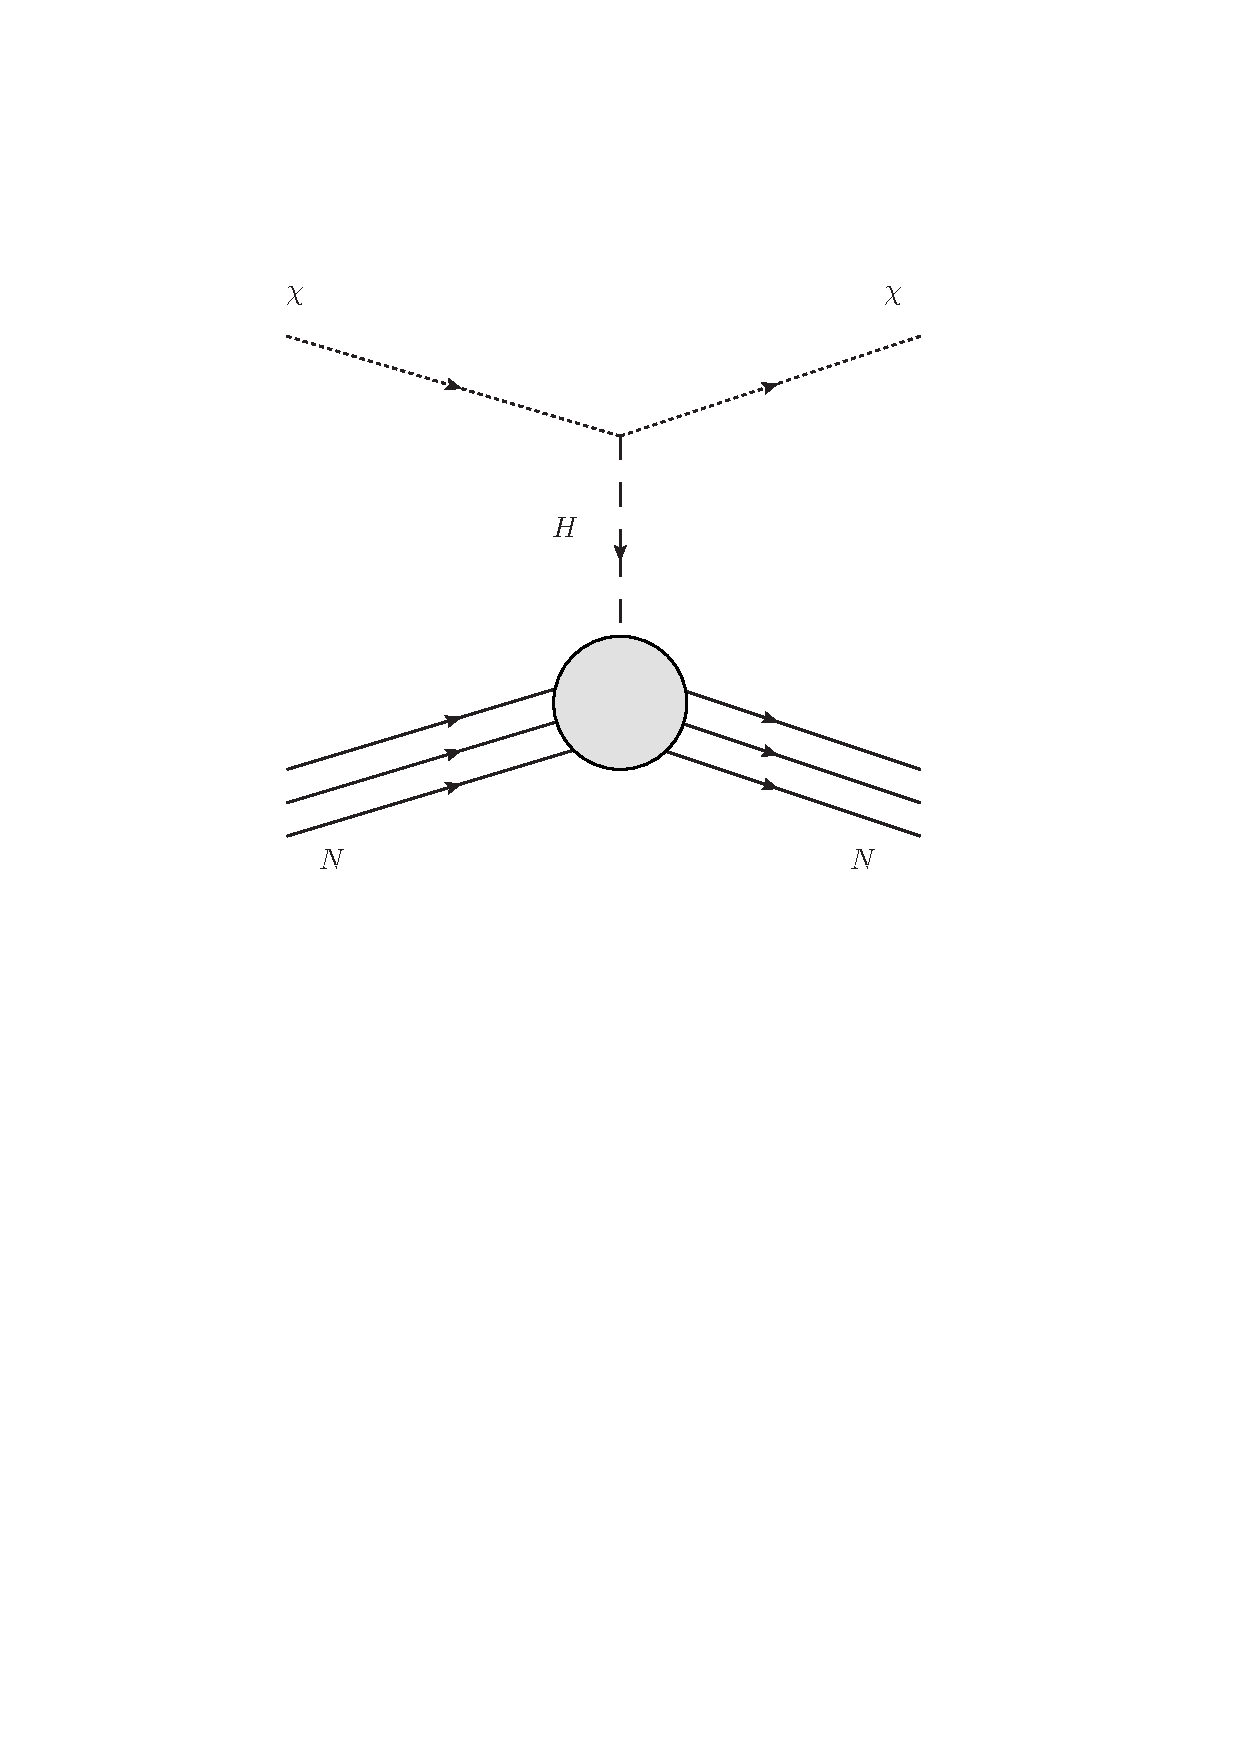
\includegraphics[width=190pt,angle=0]{Wimp_N_scattering}
\end{center}
\caption{The Higgs-boson exchange contribution to the WIMP-Nucleon low energy 
scattering process.}\label{fig:wimp_N_scatt}
\end{figure}
%

In principle lattice QCD can provide a determination of these nucleon matrix elements from first principles. 
%The difficulty involved in these computations has limited for a long time 
%the possibility to isolate a physical signal for these quantities. 
In this regard, two approaches have been followed for the calculation of the 
light and strange quark content 
of the nucleons. The first is based on the 
Feynman-Hellman theorem~\cite{Feynman:1939zz} that relates the nucleon scalar matrix 
element to the dependence of the nucleon mass on the quark masses, while the second relies on so-called ``direct method'' that involves evaluating 
the hadronic matrix elements directly.

Both approaches are numerically very challenging. In the first method, a number 
of simulations at different values of the strange quark mass are needed in order to evaluate the derivative.  
In the direct method, the computation of the disconnected diagrams is required, 
which is a highly demanding computational task. % since they often show quite a bad signal to noise 
%ratio, thus requiring very high statistics. 
In addition, as pointed out in ref.~\cite{Michael:2001bv}, when lattice 
discretizations that break chiral symmetry are used, a  
mixing between the bare light and strange scalar quark density matrix elements occurs 
under renormalization. %This mixing is not present for chiral invariant but
%it can also be avoided using, like we propose here, the gradient flow
%to define the quark scalar density in the nucleon.

Despite these challenges, there exist a number of lattice QCD computations of the strange quark 
content of the nucleon (see the review~\cite{Young:2009ps}).
Although these calculations indicate that the strange quark content of the 
nucleon is smaller than suggested from 
$\chi$PT, their quoted results are affected by large statistical errors for the reasons mentioned above.
This makes it impossible to make any definitive conclusions about the hadronic component of matrix elements that couple to DM.  To make any radical progress in this area, a novel approach to this problem is required.

\section*{Calculation of hadronic matrix elements that couple to DM probes}

This calculation is based on the possibility to relate the matrix element of 
a scalar density $\chibar_r(t,x)\chi_s(t,x)$
%strange condenstate 
%$\sbar(t,x)s(t,x)$ 
at non-vanishing flow-time between nucleon states
with the the one at vanishing flow-time.
This can be done considering the small flow-time expansion
or finding the proper WI as for the case
of the chiral condensate.
The small flow-time expansion of the scalar density 
\be
S^{rs}(t,x) = \chibar_r(t,x)\chi_s(t,x)\,,
\ee
reads
\begin{widetext}
\be
S^{rs}(t,x) = c_0(t)M^{rs} + c_1(t)M^{rs}{\rm Tr}\left[M^2\right] + c_2(t)\left(M^3\right)^{rs} + c_3(t)S^{rs}(0,x) + O(t)
\ee
\end{widetext}
where $c_0 \sim 1/t$ and $c_{1,2,3} \sim \log t$.
If one considers the subtracted matrix element
\be
\mcC^{\rm sub}(t,x) = \left\langle\mcN \mcO(t) \mcN^\dagger\right\rangle - \left\langle\mcO(t) \right\rangle \left\langle\mcN \mcN^\dagger \right\rangle
\ee
the small flow-time expansion contains only the term proportional to $c_3$
\be
\mcC^{\rm sub}(t,x) = c_3(t)\mcC^{\rm sub}(0,x)\,.
\ee
At finite flow-time no mixing is present.
To compute the physical matrix element at $t=0$ one needs to compute $c_3(t)$.
Using the chiral WIs one can show that
\be
c_3(t) = \frac{G_{\pi,t}}{G_\pi} + O(t)\,.
\ee
This implies that to compute the matrix element we are interested in we need to compute
\be
\frac{G_{\pi}}{G_{\pi,t}} \cdot \left[
\left\langle\mcN S^{rs}(t) \mcN^\dagger\right\rangle - \left\langle S^{rs}(t) \right\rangle \left\langle\mcN \mcN^\dagger \right\rangle\right]\,.
\label{eq:sbars}
\ee
We observe that the renormalization factor of $S^{rs}(t)$ simplifies with the one of $G_{\pi,t}$, thus the
only renormalization factor needed is the one for $G_\pi$, i.e. $Z_P$.
The matrix element~\eqref{eq:sbars} should be computed in a window of $t$-values,
not too small to avoid big discretization errors and not too large to avoid contributions
from higher dimensional operators. Once the continuum limit is performed at values
of $t$ fixed in physical units, the matrix element~\eqref{eq:sbars} should be 
independent of $t$ if $t$ is not too large.


\section*{CP violation within the Standard Model and electric dipole moments}
The EDMs of the neutron and proton are very sensitive probes of CP-violating sources 
beyond those contained in the SM.
In fact, the current bound on the neutron EDM strongly constrains many models of BSM physics. 
At current experimental accuracies, a nonzero nucleon EDM cannot be accounted for by the phase 
in the quark-mass matrix. 
This implies that such a signal is either caused by a nonzero QCD $\theta$ term or 
by genuine BSM physics which, at low energies, 
can be parametrized in terms of higher-dimensional CP-violating quark-gluon operators. 
Irrespective of the origin, the signal for the nucleon EDM will be small and largely 
masked by strong-interaction physics, which presents a formidable challenge to the interpretation
of such a signal.
To disentangle the origin of a nonzero EDM measurement (e.g. $\theta$ term or BSM), 
a quantitative understanding of the underlying hadronic physics is required.

In the presence of $N_f$ fermions, the general QCD Lagrangian in Euclidean space with a $\theta$ term
reads
\begin{equation}
{\cal L_\theta}= {1\over 4} F_{\mu\nu}^a(x)F_{\mu\nu}^a(x)
+ \bar\psi\, D \psi
+ \bar\psi_L \,M\,\psi_R + \bar\psi_R \,M^\dagger\,\psi_L
- i \theta_q q(x),
\end{equation}
%\begin{equation}\label{QCD1}
%\mathcal L_{\mathrm{QCD}} = -\frac{1}{4}G_{\mu\nu}^aG^{a,\mu\nu} + \bar\Psi(i\Dslash{D} - M)\Psi - \theta_q \frac{g^2}{64\pi^2}\epsilon^{\mu\nu\alpha\beta} G^a_{\mu \nu}G^a_{\alpha \beta}\,\,\,,
%\end{equation}
where $\psi$ is an $N_f$ component vector in flavor space, $M$ is the
quark mass matrix, and $q(x)$ is the topological charge density.  The parameter
$\theta_q$ and the imaginary part of the quark mass are related, so that the
relevant $\theta$ parameter is given by
\begin{equation}
\theta = \theta_q + {\rm arg}\,{\rm det}\, M.
\label{thetafe}
\end{equation} 
This term is CP-violating and induces, for example,  an electric dipole moment within the neutron.    
One of the most stringent constraints on possible violations of parity and time reversal 
(equivalently CP symmetry assuming CPT invariance) symmetries is inferred from
measurements of the neutron EDM.  

\section*{The Gradient flow}

In this section we give a short introduction to the gradient flow that is at the base of the
method we propose to use for this project.
The gradient flow (GF), for gauge~\cite{Luscher:2010iy} 
and fermion~\cite{Luscher:2013cpa} fields, used in combination with a lattice regulator, 
can probe the non-perturbative dynamics of QCD
in advantageous manners.
It is defined by a differential equation that gauge and fermion
fields satisfy as a function of the space-time coordinates $x$ and of a new
scale, the flow time $t$.

The works by L\"uscher and Weisz~\cite{Luscher:2010iy,Luscher:2011bx,Luscher:2013cpa}
give us a complete understanding of the continuum limit
of observables at non-vanishing flow time. This allows us to use the GF
to define observables that otherwise would be difficult
to compute with standard methods.
For example the GF has been used to give operational definitions to the
fundamental parameters of QCD as the strong coupling~\cite{Luscher:2010iy,Fodor:2012td,Fritzsch:2013je}
or other quantities, as the chiral condensate~\cite{Luscher:2013cpa}
and the energy-momentum tensor~\cite{Suzuki:2013gza,DelDebbio:2013zaa}.
The GF can also be used to define new relative ways to set the scale in 
lattice QCD calculations~\cite{Luscher:2010iy,Borsanyi:2012zs}.

In particular the topological susceptibility~\cite{Luscher:2010iy} and the chiral condensate~\cite{Luscher:2013cpa}
can be computed with rather high precision because with the gradient flow 
mixing with lower-dimensional operators can be avoided.
Local operators at non-vanishing flow time have a very simple renormalization pattern~\cite{Luscher:2010iy,Luscher:2011bx,Luscher:2013cpa},
but to relate them with the operators at vanishing flow time one has to rely to 
Ward identities (WI)~\cite{Luscher:2013cpa,DelDebbio:2013zaa,Shindler:2013bia} or to the small flow-time expansion.

The goal of this project to perform the matching of the correlation functions computed at non-zero
flow time with the physical quantities such as the EDM, the strange content of the nucleon 
or, as a test ground, the energy.

The results will be published in scientific journals, if possible.

\section*{Progress plan and milestones}
The aims and progress plan of this thesis are as follows
\begin{itemize}
\item Fall 2xxx: study the gradient flow for gauge fields~\cite{Luscher:2010iy} and fermions~\cite{Luscher:2013cpa}.
\item Fall 2xxx: development of gauge field Feynman rules with the gradient flow.
\item Fall 2xxx and Spring 2xxx: perturbative calculation of the energy defined with the gradient flow (this can be matched
with the non-perturbative calculation to extract the $\Lambda_{\rm QCD}$ parameter).
\item Spring 2xxx: development of Feynman rules for fermion fields at non-zero flow time.
\item Spring 2xxx: sample perturbative calculation with fermions (quark propagator, fermion bilinears)
\item Spring 2xxx: The last part deals with a proper write-up of the thesis. 
\end{itemize}
 

The thesis is expected to be handed in May/June 2xxx.


%\bibliographystyle{apsrev}
\bibliography{references}



\end{document}
